\subsection{Un enjeu central : mieux connaître les auditeurs}

Les réflexions conduites dans le cadre de cette étude font émerger un constat central :

\begin{quote}
\textbf{Le potentiel des auditeurs IHEDN apparaît significatif, mais demeure aujourd'hui insuffisamment identifié et structuré.}
\end{quote}

Si l'IHEDN dispose historiquement d'un réseau dense et diversifié de compétences, les capacités concrètes de mobilisation des auditeurs restent imparfaitement objectivées. L'annuaire existant demeure en effet lacunaire et ne permet pas, en l'état, d'identifier avec suffisamment de précision les compétences susceptibles d'être utiles dans une démarche de préparation, d'analyse ou de retour d'expérience.

L'examen de l'annuaire papier 2022 confirme cette limite\footnote{Analyse interne réalisée par Bruno Leray à partir de l'annuaire papier 2022 des anciens auditeurs et membres associés de l'IHEDN.}. La communauté recensée y apparaît particulièrement large, avec environ 28\,000 anciens auditeurs, et près de 30\,000 personnes en incluant les membres associés. Les adhérents des \AssociationsUnionIHEDN{} ne représentent toutefois qu'une fraction minoritaire de cet ensemble.

Les données disponibles permettent ainsi d'apprécier un périmètre d'appartenance ou d'adhésion ; elles ne permettent pas, en revanche, de connaître l'activité effective des membres, leurs capacités mobilisables, leurs contraintes de disponibilité, les raisons de leur engagement associatif ou encore leur motivation.

\clearpage

\begin{table}[H]
\centering
\small
\setlength{\tabcolsep}{4pt}
\begin{tabularx}{\linewidth}{@{}p{4.4cm}Yp{3.2cm}@{}}
\toprule
\textbf{Périmètre observé} & \textbf{Ordre de grandeur issu de l'annuaire 2022} & \textbf{Enseignement pour le questionnaire} \\
\midrule
Communauté IHEDN recensée & Environ 28\,000 anciens auditeurs, et près de 30\,000 personnes en incluant les membres associés. & Le vivier théorique recensé par l'annuaire dépasse largement le périmètre des membres effectivement engagés dans les \AssociationsUnionIHEDN. \\
\addlinespace
Adhérents des \AssociationsUnionIHEDN{} & Environ 5\,470 adhérents au total, dont près de 3\,250 adhérents au sein des associations régionales. & Le questionnaire administré aux adhérents ne couvre qu'une fraction minoritaire des anciens auditeurs. \\
\addlinespace
Poids relatif de l'adhésion & Rapportés aux quelque 28\,000 anciens auditeurs recensés, les quelque 5\,470 auditeurs adhérents représentent environ 19,5\%. & Les résultats devront être interprétés comme une mesure du potentiel associatif, non comme une photographie exhaustive de toute la communauté IHEDN. \\
\addlinespace
Associations régionales & Les effectifs varient fortement selon les territoires, d'une vingtaine de membres à environ 380 pour l'\ARSeize. & Le dispositif devra tenir compte des écarts de taille, de dynamique associative et de capacité de réponse. \\
\bottomrule
\end{tabularx}
\caption{Éléments de cadrage issus de l'annuaire IHEDN 2022.}
\label{tab:cadrage_annuaire_2022}
\end{table}

\clearpage

La figure \ref{fig:comparaison_repartition_categories} présente la répartition des adhérents et des auditeurs selon les différentes catégories de formation IHEDN.

\begin{figure}[htbp]
    \centering

    \begin{subfigure}[b]{0.48\textwidth}
        \centering
        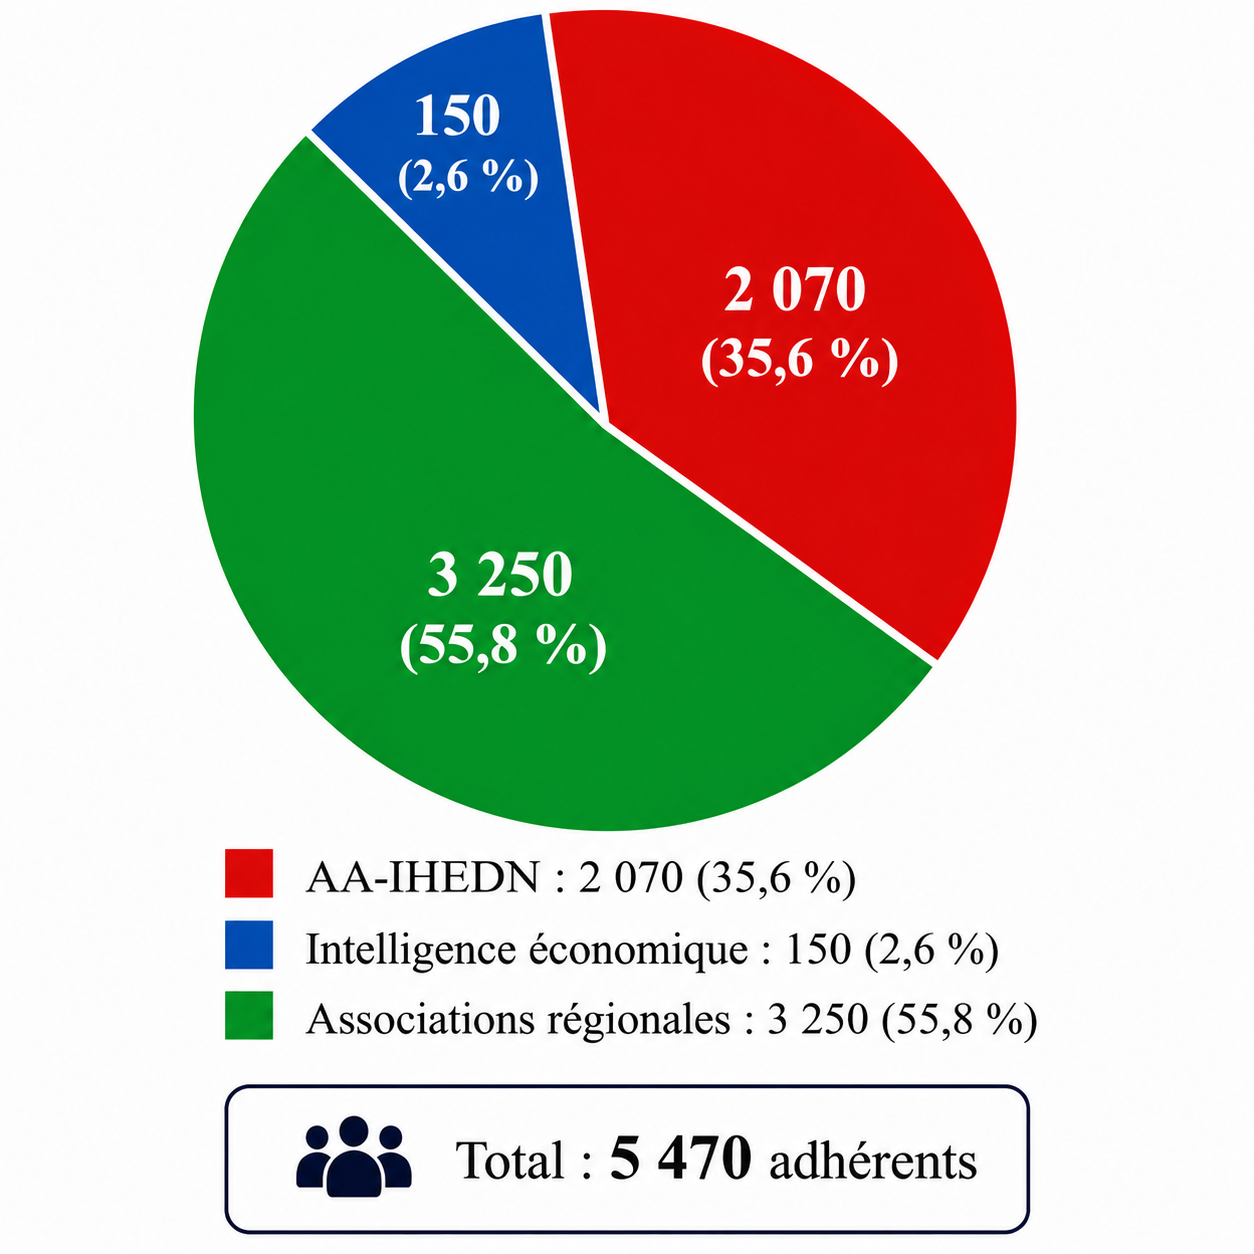
\includegraphics[width=\textwidth]{Figures/repartition_adherents_par_categorie}
        \caption{Répartition des adhérents par catégorie}
        \label{fig:repartition_adherents}
    \end{subfigure}
    \hfill
    \begin{subfigure}[b]{0.48\textwidth}
        \centering
        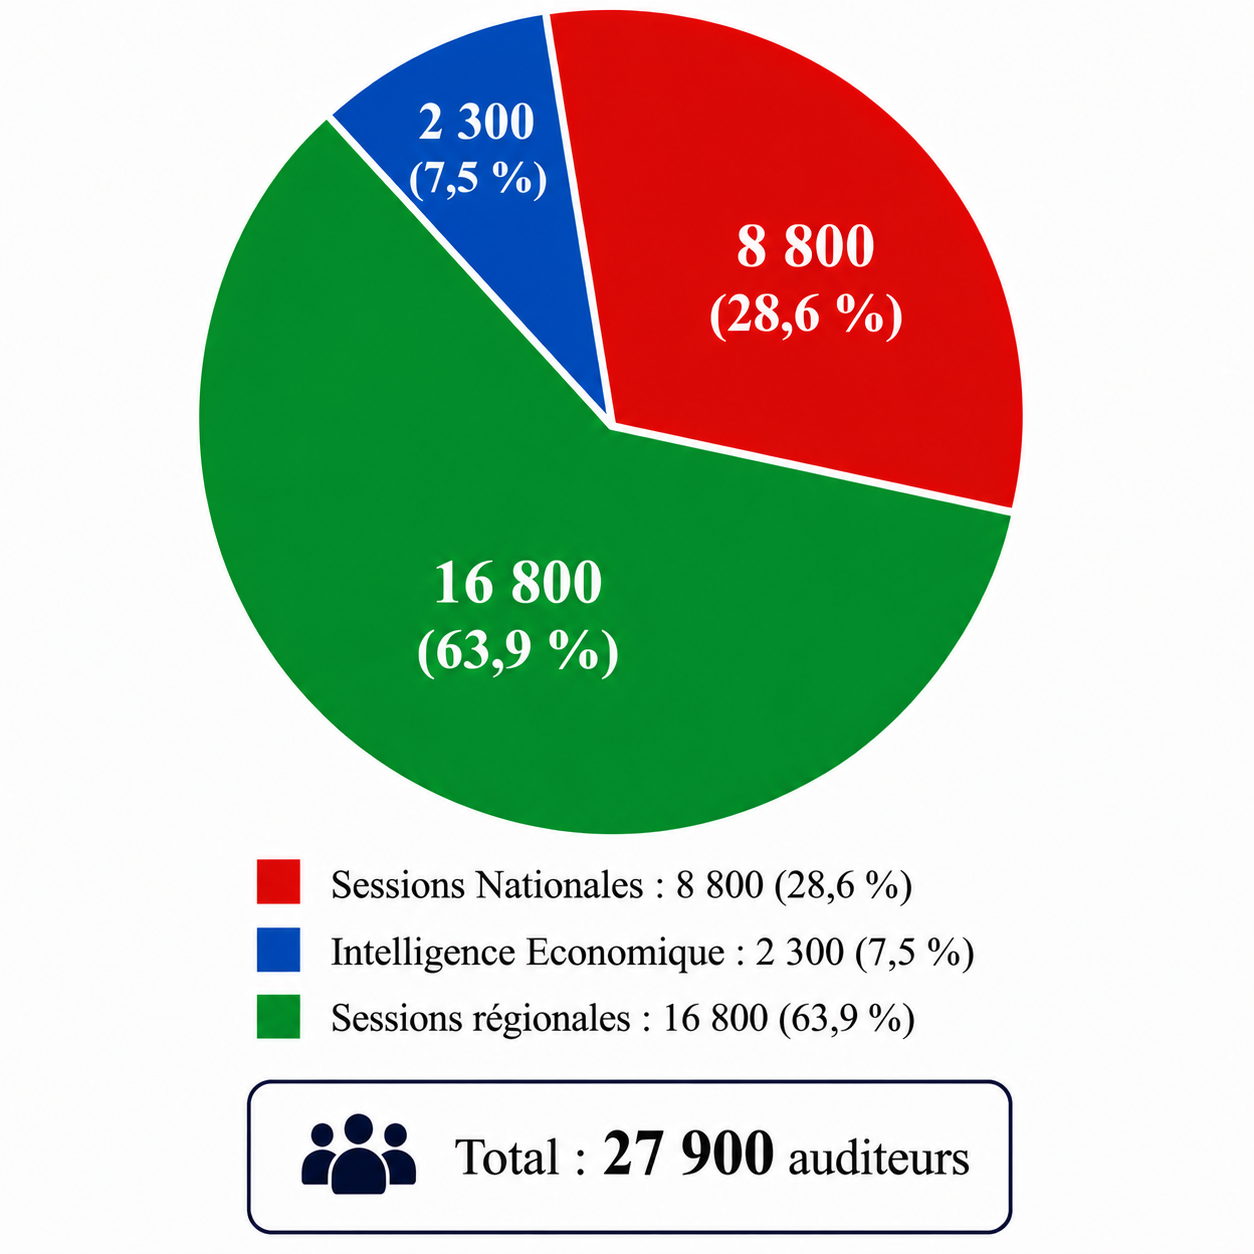
\includegraphics[width=\textwidth]{Figures/repartition_auditeurs_par_categorie}
        \caption{Répartition des auditeurs par catégorie}
        \label{fig:repartition_auditeurs}
    \end{subfigure}

    \caption{Comparaison de la répartition des adhérents et des auditeurs selon les différentes catégories de formation IHEDN.}
    \label{fig:comparaison_repartition_categories}
\end{figure}

Ces données mettent en évidence un premier constat structurant : le nombre d'adhérents effectivement engagés dans les associations d'anciens auditeurs demeure relativement limité au regard du volume total des auditeurs formés par l'IHEDN depuis l'origine.

Ce constat conduit à relativiser fortement l'idée d'un vivier immédiatement mobilisable de plusieurs dizaines de milliers de personnes.

Même parmi les sessions les plus récentes, une majorité d'auditeurs ne s'engage pas dans une \AssociationUnionIHEDN. Le taux d'adhésion observé ne doit donc pas être interprété comme un simple indicateur d'appartenance, mais comme un indice partiel du maintien d'un lien associatif après la session.

Par ailleurs, ces chiffres doivent être interprétés avec prudence. L'annuaire ne distingue pas les auditeurs décédés et agrège l'ensemble des promotions depuis les origines des sessions nationales et régionales. Le vivier théorique présenté par l'annuaire ne correspond donc pas nécessairement à une capacité réelle d'engagement.

Cette distinction entre potentiel théorique et potentiel effectivement mobilisable constitue un enjeu central de la réflexion.

L'annuaire fait également apparaître une érosion de l'adhésion avec l'ancienneté des sessions, phénomène qui peut tenir à l'âge, à l'évolution des disponibilités, aux trajectoires professionnelles ou encore à l'intensité variable du lien associatif.

Ce constat ne relève pas uniquement d'une donnée démographique. Il souligne l'intérêt de mieux comprendre les ressorts de l'adhésion, les causes de son érosion et les formes concrètes d'engagement dans les activités associatives.

\clearpage

\subsubsection{Évolution des taux d'adhésion selon les générations d'auditeurs}

Pour les sessions régionales, l'analyse des données fait apparaître une progression importante du taux d'adhésion parmi les promotions les plus récentes, comme en témoigne la figure \ref{fig:adhesion_sr}.

\begin{figure}[H]
    \centering
    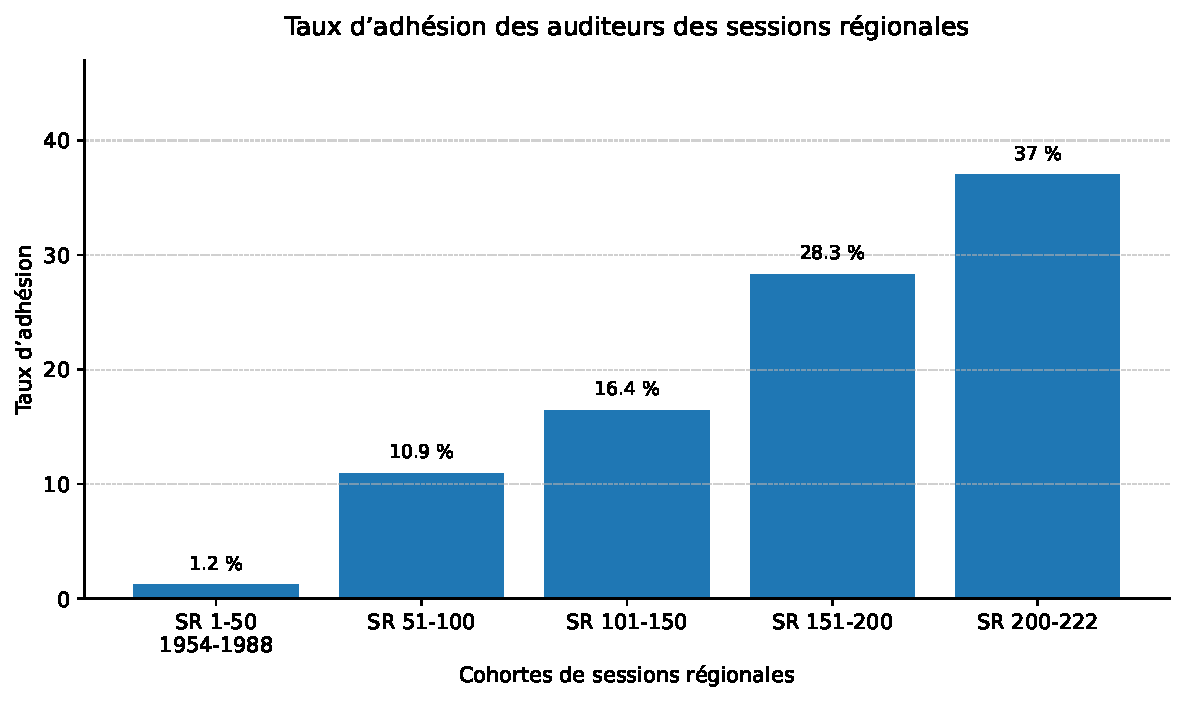
\includegraphics[width=0.85\linewidth]{Figures/graphe_adhesion_sr.pdf}
    \caption{Évolution du taux d'adhésion des auditeurs des sessions régionales selon les cohortes de sessions.}
    \label{fig:adhesion_sr}
\end{figure}

Les sessions régionales les plus anciennes affichent des taux d'adhésion particulièrement faibles, tandis que les promotions plus récentes conservent généralement un lien plus étroit avec leur association régionale de rattachement. Cette diminution progressive du taux d'adhésion au fil du temps semble ainsi largement corrélée au vieillissement des auditeurs.

À titre indicatif, les participants des sessions régionales 123 (1995), 143 (2000), 160 (2005), 180 (2010), 200 (2015) et 219 (2020) étaient âgés de 35 à 55 ans au moment de leur formation. En 2025, les auditeurs de la session régionale 123 auraient ainsi entre 65 et 95 ans, tandis que ceux de la session régionale 160 seraient âgés de 55 à 75 ans.

Cette évolution démographique contribue vraisemblablement à expliquer l'érosion des effectifs adhérents. Elle s'accompagne en effet de transformations des disponibilités personnelles et professionnelles, mais également d'un affaiblissement progressif des réseaux de sociabilité constitués à l'occasion des sessions, lesquels tendent naturellement à se distendre avec le temps.

L'analyse des sessions nationales, illustrée sur la figure \ref{fig:adhesion_sn}, met également en évidence des taux d'adhésion globalement plus élevés.

\begin{figure}[H]
    \centering
    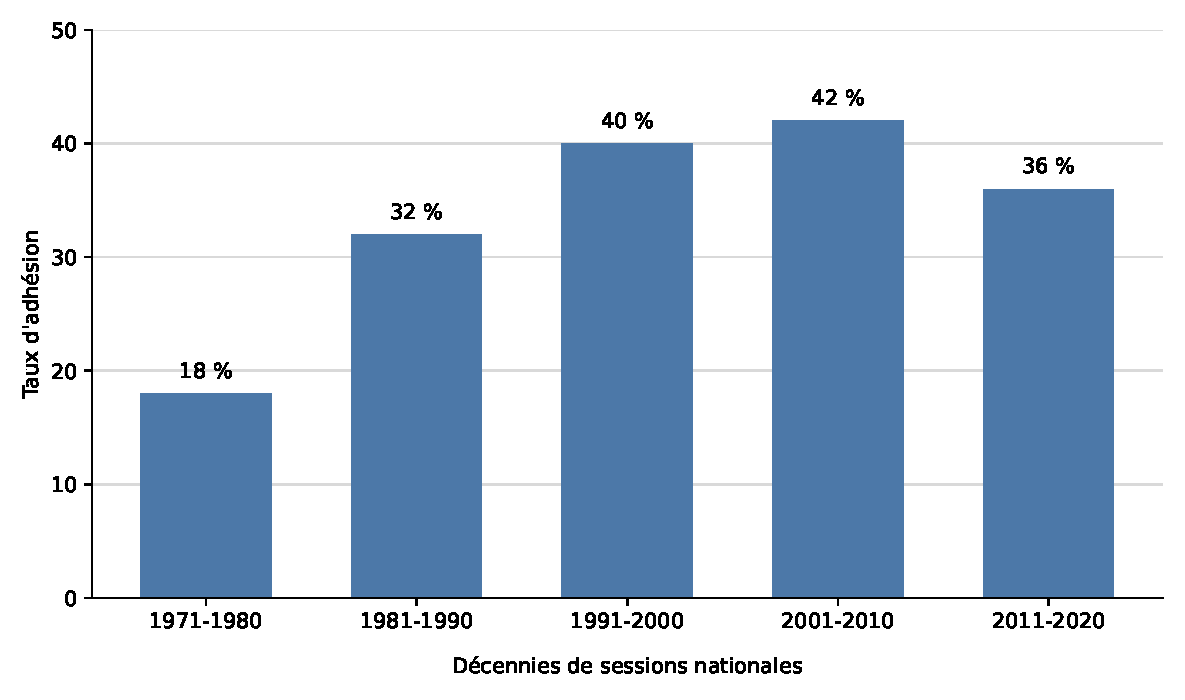
\includegraphics[width=0.85\linewidth]{Figures/graphe_adhesion_sn.pdf}
    \caption{Évolution du taux d'adhésion des auditeurs des sessions nationales selon les décennies.}
    \label{fig:adhesion_sn}
\end{figure}

Les auditeurs des sessions nationales apparaissent davantage enclins à adhérer à leur association dédiée. Cette situation peut notamment s'expliquer par la centralité institutionnelle des sessions nationales, des logiques de réseau professionnel plus fortes, une sociabilité plus durable ainsi que par le prestige associé à ces formations.

\subsubsection{Une structuration territoriale inégale des associations régionales}

Les données disponibles mettent également en évidence une forte hétérogénéité entre les associations régionales. Leurs effectifs sur le territoire métropolitain varient d'une vingtaine de membres pour l'AR~5 -- Bretagne occidentale à environ 380 membres pour l'\ARSeize{} -- Paris--Île-de-France.

Les associations régionales les plus importantes, c'est-à-dire comptant plus de 100 membres, sont notamment\footnote{La liste complète des \AssociationsRegionalesIHEDN{} ainsi que la localisation de leur siège sont présentées en annexe \ref{annexe:maillage_territorial_ihedn}.} :
\begin{itemize}
    \item l'\ARSeize{} -- Paris--Île-de-France ;
    \item l'AR~14 -- Région lyonnaise (environ 300 membres) ;
    \item l'AR~1 -- Aquitaine (environ 220 membres) ;
    \item l'AR~7 -- Centre-Val de Loire (environ 180 membres) ;
    \item les AR~2 -- Auvergne, 10 -- Franche-Comté, 15 -- Région Nord et 19 -- Occitanie Pyrénées (environ 140 membres) ;
    \item les AR~9 -- Provence et 12 -- Languedoc-Roussillon (environ 120 membres) ;
    \item les AR~6 -- Haute Bretagne, 8 -- Dauphiné-Savoie, 13 -- Lorraine, 18 -- Poitou-Charentes, 21 -- Versailles--Yvelines--Hauts-de-Seine, 22 -- Alsace et 29 -- Nice Côte d'Azur (environ 100 membres).
\end{itemize}

Les autres associations régionales comptent généralement moins de 60 membres.

La figure \ref{fig:carte_AR} présente la répartition territoriale des associations régionales en fonction de leurs effectifs approximatifs.

\begin{figure}[H]
\centering
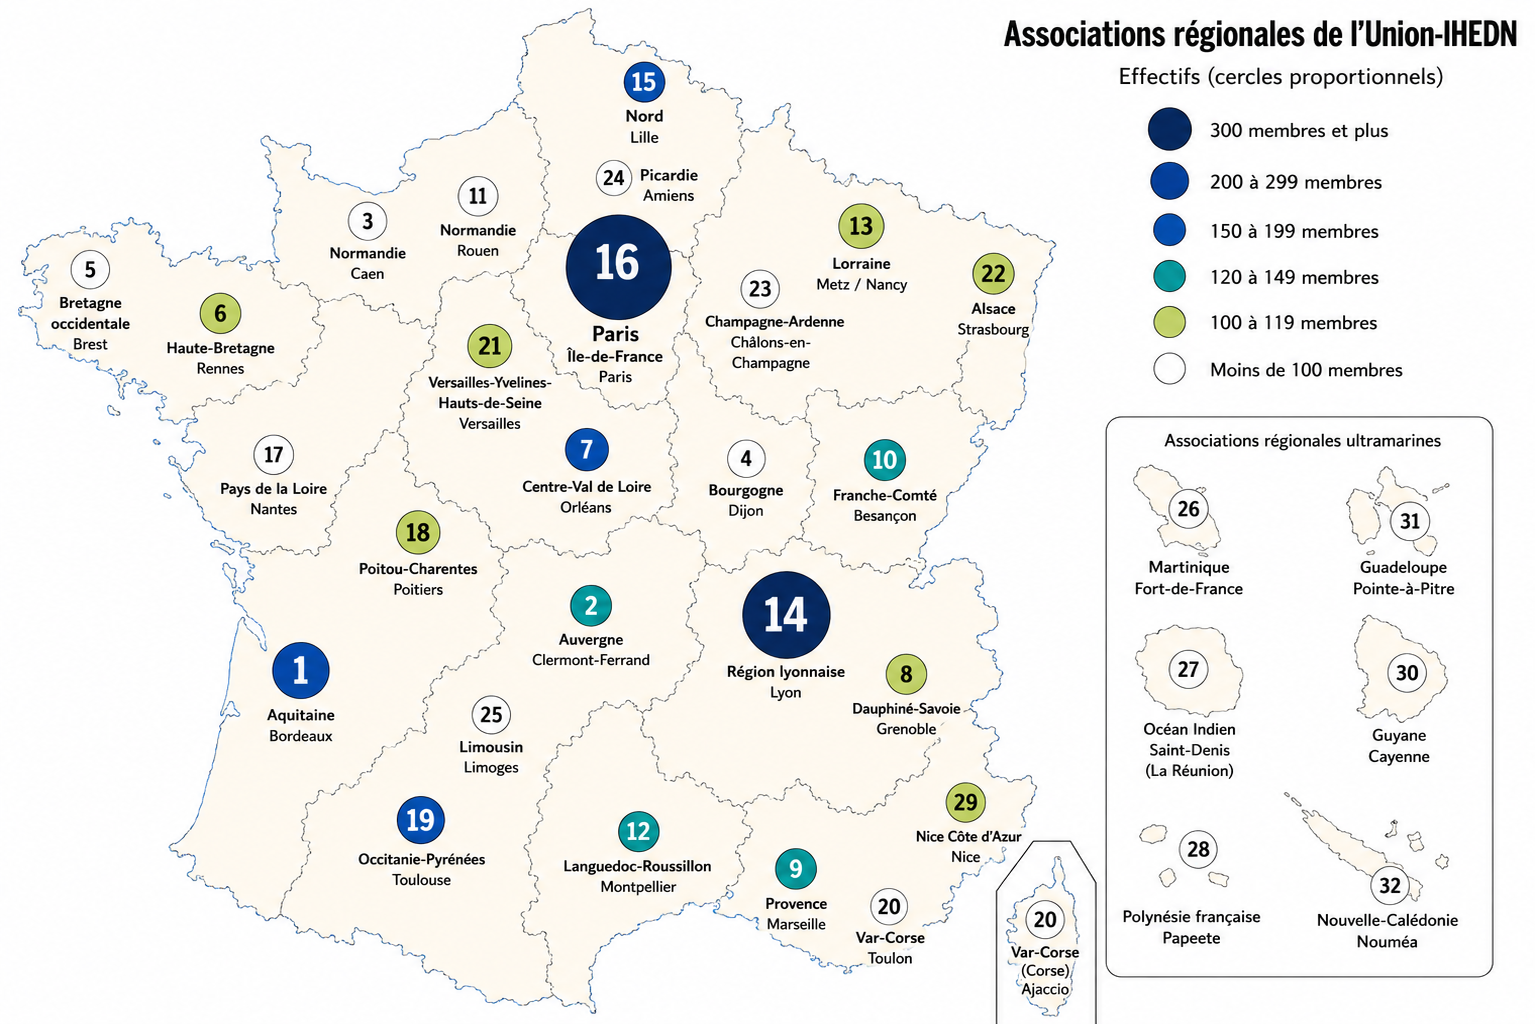
\includegraphics[width=\linewidth]{Figures/carte_AR}
\caption{Répartition territoriale des \AssociationsRegionalesIHEDN{} et importance relative de leurs effectifs.}
\label{fig:carte_AR}
\end{figure}

Cette dispersion des effectifs invite à distinguer le vivier national théorique, constitué par l'ensemble des quelque 28\,000 anciens auditeurs, du vivier associatif réellement atteignable par une enquête administrée aux seuls adhérents.

Elle conduit également à poser explicitement la question du périmètre de l'étude : celui-ci pourrait être celui des personnes sensibilisées aux enjeux de défense, soit l'ensemble des anciens auditeurs recensés. Toutefois, dans un premier temps, l'enquête envisagée vise principalement à objectiver les capacités réelles du périmètre associatif effectivement mobilisable.

L'annuaire ne renseigne pas sur l'activité effective des adhérents au sein des associations. Seule une enquête auprès des membres permettrait ainsi de mieux comprendre les ressorts de l'adhésion et de son érosion, mais également les conditions concrètes de l'engagement effectif dans les activités associatives.

Cette limite empêche de valoriser pleinement les capacités potentielles du réseau des auditeurs. La mise en place d'un outil dédié apparaît dès lors comme une étape préalable indispensable pour mieux connaître les profils, apprécier les disponibilités réelles et définir, le cas échéant, des formes d'implication adaptées aux différentes temporalités de la gestion de crise.

\clearpage

\subsection{Une démarche d'objectivation}

Le comité propose de recourir à un questionnaire afin de disposer d'une connaissance plus fiable et plus exploitable des membres. Il ne s'agit ni d'une simple actualisation administrative, ni d'une opération de communication, mais d'un instrument destiné à mieux apprécier les ressources humaines, les expertises et les motivations susceptibles d'être mobilisées au sein des \AssociationsUnionIHEDN.

Cette réflexion s'inscrit dans la continuité de travaux antérieurs relatifs à la création d'une réserve, étudiée à la demande d'Édouard Philippe en 2015\footcite{DESAINTSALVY2026}. Elle trouve également un écho dans des analyses récentes émanant de personnalités de premier plan au sein de l'IHEDN. Anne-François de Saint Salvy (Vice-amiral d'escadre (2S) et Vice-président de l'Association des anciens auditeurs de l'IHEDN) souligne ainsi, dans son article « Comment mobiliser les auditeurs de l'IHEDN ? » paru en mars 2026\footcite{DESAINTSALVY2026} :

\begin{quote}
« Il est temps aujourd'hui de reprendre ce projet, sans doute d'une manière simplifiée et de se mettre en mesure de tirer profit des multiples compétences qu'apportent les auditeurs de l'IHEDN. Au-delà d'un statut et d'une organisation, le premier pas est sans doute celui d'un recensement des compétences disponibles, inscrites dans une grille permettant de les utiliser efficacement et tenu à jour régulièrement. »
\end{quote}

Cette démarche s'inscrit par ailleurs dans un contexte institutionnel marqué par un intérêt croissant pour la contribution des citoyens engagés et des réseaux associatifs à la préparation et à la gestion des crises majeures. La lettre adressée par l'IHEMI le 30 décembre 2025 relative aux enjeux liés aux risques et aux crises illustre cette dynamique\footcite{IHEMI:2025:LIREC75}. Elle souligne l'intérêt de mieux identifier et valoriser les ressources disponibles au sein des réseaux d'acteurs engagés afin de renforcer leur contribution aux actions de sensibilisation, de préparation, d'analyse et de retour d'expérience.

Dans cette perspective, le questionnaire proposé par le comité constitue un premier outil permettant de transformer cette ambition en une démarche concrète de connaissance et de structuration des ressources disponibles. Il vise à recueillir des données qualitatives et quantitatives utiles pour apprécier les formes possibles d'implication des membres des \AssociationsUnionIHEDN et à fournir une base objective pour orienter les réflexions futures de l'association.

Cette démarche pourrait s'inscrire dans le cadre du cinquantième anniversaire de l'\UnionIHEDN. Cette échéance offre un cadre particulièrement propice pour engager une réflexion collective sur l'histoire de l'association, ses ressources et sa capacité d'adaptation face aux défis contemporains.

Avant d'engager un tel projet, le comité a d'abord précisé les objectifs assignés au questionnaire.

\clearpage

\subsection{Objectifs du questionnaire}

Le questionnaire vise à cartographier les compétences, identifier les disponibilités et structurer une base de données exploitable. Les principaux objectifs opérationnels associés à cette démarche sont présentés dans le tableau \ref{tab:objectifs_questionnaire}.

\begin{table}[H]
\centering
\footnotesize
\setlength{\tabcolsep}{4pt}

\resizebox{\linewidth}{!}{%
\begin{tabular}{@{}>{\raggedright\arraybackslash}p{4cm}>{\raggedright\arraybackslash}p{7.5cm}>{\raggedright\arraybackslash}p{5.5cm}@{}}
\toprule

\textbf{Axe d'action} &
\textbf{Proposition} &
\textbf{Objectif} \\

\midrule

Cartographie des compétences &
Élaborer et diffuser un questionnaire auprès des adhérents des associations afin d'identifier leurs domaines d'expertise, leurs compétences, leurs disponibilités déclarées et leurs formes possibles de contribution. &
Disposer d'une vision consolidée et réaliste du potentiel associatif. \\

\addlinespace

Base de données centralisée &
Constituer une base de données regroupant les compétences identifiées, exploitable par les associations dans un cadre conforme aux règles de protection des données. &
Faciliter la préparation, l'analyse et le dialogue institutionnel, sans présumer d'une mobilisation opérationnelle. \\

\addlinespace

Hypothèse de dispositif d'appui &
Étudier, à partir des données recueillies, les conditions et les limites d'un éventuel dispositif d'appui associatif, en lien avec les instances de l'IHEDN et les autorités compétentes. &
Apprécier les formes de contribution envisageables sans créer de chaîne autonome de gestion de crise. \\

\addlinespace

Analyse du dispositif antérieur &
Analyser les raisons ayant conduit à l'interruption de la précédente réserve des auditeurs. &
Tirer les enseignements nécessaires avant toute réactivation. \\

\addlinespace

Identification des formes d'engagement &
Identifier les membres volontaires, les domaines dans lesquels ils accepteraient de contribuer et les contraintes qui encadrent cette disponibilité. &
Assurer la crédibilité du dispositif et éviter toute surestimation des capacités réelles. \\

\bottomrule
\end{tabular}
}

\caption[Objectifs structurants du questionnaire]{Objectifs structurants associés à la mise en place du questionnaire de cartographie des compétences des auditeurs IHEDN.}
\label{tab:objectifs_questionnaire}

\end{table}

\begin{proposition}{Mettre en place un questionnaire de cartographie des compétences}
Le comité propose l'élaboration et la diffusion d'un questionnaire visant à identifier les compétences, les disponibilités et les capacités potentielles de contribution des adhérents des associations en matière de résilience et de gestion des crises majeures.
\end{proposition}

\begin{proposition}{Structurer une base de données des compétences mobilisables}
Les informations recueillies pourraient permettre la constitution d'une base de données des compétences, destinée à mieux identifier les ressources disponibles dans le cadre d'actions de préparation, d'analyse ou de \acrshort{retex}.
\end{proposition}

Dans la perspective de concevoir ce questionnaire, le comité a fait appel à l'expertise du docteur Victor Violier, sociologue à l'\gls{irsem}\footcite{violier_irsem}, afin de disposer de fondements méthodologiques solides et d'en encadrer la mise en \oe{}uvre\footnote{Entretien avec le docteur Victor Violier, sociologue à l'IRSEM, réalisé le 20 février 2026}.

\clearpage

\subsection{Cadre méthodologique}

Sur la base des conseils du docteur Violier, la démarche doit s'inscrire dans une logique sociologique d'objectivation des données, afin de dépasser les représentations spontanées\footnote{\textit{Ibid.}}.

Les données issues de l'annuaire 2022 invitent à préciser le périmètre de l'enquête. Si le questionnaire est adressé aux seuls adhérents, il mesurera d'abord la capacité d'engagement des \AssociationsUnionIHEDN. S'il devait être étendu à un cercle plus large d'anciens auditeurs, il poserait d'autres difficultés : accès aux coordonnées, actualisation des fichiers, statut des personnes inactives ou décédées, conformité juridique et interprétation des non-réponses. Le comité retient donc une approche progressive, centrée sur un périmètre maîtrisable, tout en signalant explicitement les limites de représentativité qui en découlent.

La construction du questionnaire devra respecter plusieurs principes méthodologiques. Il conviendra d'abord d'éviter toute imposition de problématique\footcite{Bourdieu1986}, en formulant des questions neutres et non orientées, afin de ne pas influencer les réponses et de préserver la fiabilité des données recueillies. Il faudra également tenir compte du risque d'« illusion biographique », entendue, au sens de Pierre Bourdieu, comme la tendance des individus à reconstruire \textit{a posteriori} leur trajectoire de manière cohérente et linéaire\footcite[69]{Bourdieu1986}. Dans le cadre du questionnaire, ce biais peut conduire les répondants à surestimer la cohérence de leur parcours ou à présenter leurs compétences de manière rétrospectivement rationalisée, au détriment d'une description plus nuancée de leurs expériences et de leurs capacités réelles. Enfin, une attention particulière devra être portée à l'équilibre entre questions ouvertes et questions fermées\footcite[65]{Fenneteau2015}.

Sur le plan juridique, la démarche devra être conforme au \gls{rgpd}\footcite{RGPD_CNIL}, ainsi qu'aux exigences en matière de protection des données et aux principes d'anonymisation.

\begin{proposition}{Garantir un encadrement méthodologique et juridique du questionnaire}
Le comité considère que la conception du questionnaire doit reposer sur une méthodologie rigoureuse, fondée sur des principes d'objectivation des données, de neutralité des questions et de clarification du périmètre enquêté, tout en garantissant la conformité du dispositif au \gls{rgpd} et aux exigences de protection des données personnelles.
\end{proposition}

La mise en place de ce questionnaire permettrait à l'association de disposer d'éléments plus concrets pour préciser son rôle, documenter ses compétences internes et, le cas échéant, présenter une contribution lisible aux différents niveaux des associations et de l'IHEDN. La question de sa diffusion vers les autorités publiques et de sa reconnaissance institutionnelle constitue dès lors le prolongement de cette démarche.
\clearpage

\subsection{Assurer une reconnaissance institutionnelle}

Le premier apport de ce questionnaire réside dans la production d'une base factuelle susceptible de renforcer la lisibilité des associations et de leurs membres.

Toute relation utile avec les acteurs de la gestion de crise suppose une identification claire, un cadre d'action défini et une utilité reconnue par les autorités. Ces trois éléments constituent le socle de la démarche.

Disposer d'éléments factuels permettra d'étayer les échanges avec préfets, maires et acteurs de la sécurité civile, d'examiner les conditions d'une articulation avec les dispositifs existants et d'explorer un éventuel partenariat avec les \gls{dmd}\footcite{DMD_def_missions}.

\begin{proposition}{Renforcer la lisibilité institutionnelle des \AssociationsUnionIHEDN}
Le comité considère que le questionnaire pourrait constituer un outil de structuration et de légitimation des compétences disponibles au sein des \AssociationsUnionIHEDN, afin de faciliter le dialogue avec les autorités publiques, d'améliorer la lisibilité du réseau associatif et d'examiner les conditions d'une articulation avec les dispositifs existants de gestion de crise.
\end{proposition}

Au regard de l'ensemble des éléments présentés, le comité a également souhaité établir un calendrier prévisionnel de mise en \oe{}uvre du questionnaire.